\documentclass[12pt, twoside]{article}
\usepackage[letterpaper, margin=1in, headsep=0.5in]{geometry}
\usepackage[english]{babel}
\usepackage[utf8]{inputenc}
\usepackage{amsmath}
\usepackage{amsfonts}
\usepackage{amssymb}
\usepackage{tikz}
\usetikzlibrary{quotes, angles}
\usepackage{graphicx}
\usepackage{enumitem}
\usepackage{multicol}

\newif\ifmeta
\metatrue %print standards and topics tags

\title{Regents Geometry}
\author{Chris Huson}
\date{September 2020}

\usepackage{fancyhdr}
\pagestyle{fancy}
\fancyhf{}
\renewcommand{\headrulewidth}{0pt} % disable the underline of the header
\raggedbottom


\fancyhead[LE]{\thepage}
\fancyhead[RO]{\thepage \\ Name: \hspace{4cm} \,\\}
\fancyhead[LO]{BECA / Dr. Huson / Geometry 08-Area+volume\\* pset ID: 126}

\begin{document}

\subsubsection*{8-12DN-Compound-volume}
\begin{enumerate}
\item Find the area of the shape shown below composed of a rectangle and triangle with a semi-circle cut out.
    \begin{flushright}
    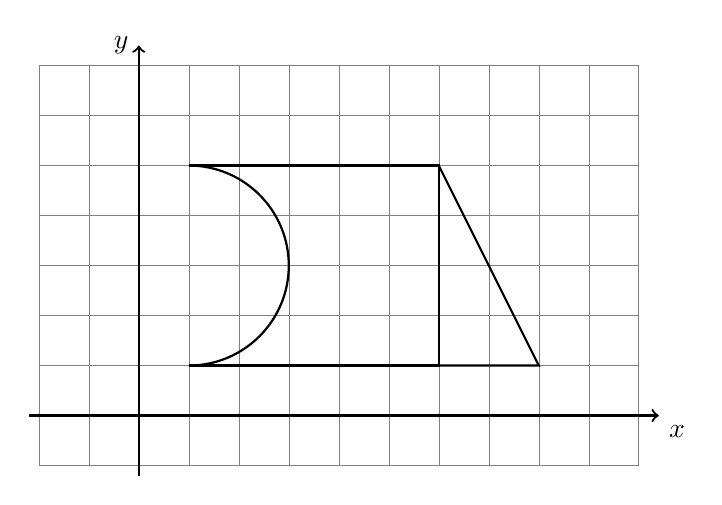
\begin{tikzpicture}[scale=.635]
      \draw [help lines] (-2,-1) grid (10,7);
      \draw [thick, ->] (-2.2,0) -- (10.4,0) node [below right] {$x$};
      \draw [thick, ->] (0,-1.2)--(0,7.4) node [left] {$y$};
      \draw [thick] (1,1)--(6,1)--(6,5)--(1,5);
      \draw [thick] (6,1)--(8,1)--(6,5);
      %\draw [thick] (1,1)--(-1,3)--(1,5);
      \draw [thick] (1,1) arc (-90:90:2);
    \end{tikzpicture}
  \end{flushright} \vspace{2cm}
  
\item Circle $O$ has a radius $AO=10$, as shown below, and $m\angle AOB=120^\circ$.
  \begin{enumerate}
    %\item Find the arc measure $m \wideparen{AB}$. \vspace{1.5cm}
    \item Find the length of the arc $\wideparen{AB}$. %\vspace{3.5cm}
      \begin{flushright}
      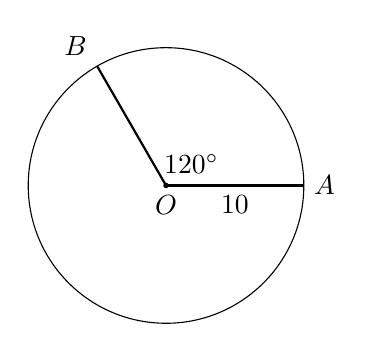
\begin{tikzpicture}[scale=.35]
        \draw (0,0) circle[radius=5];
        \draw [thick]
        (0:5) node[right] {$A$}--(0,0);
        \draw [thick] (0,0)--(120:5) node[above left] {$B$};
        \fill (0,0) circle[radius=0.1] node[below]{$O$};
        \draw (40:1.2) node{$120^\circ$};
        \draw (0:2.5) node[below]{$10$};
        %\draw (75:1.8) node[above] {$C$};
        %\draw (290:5) node[below] {$D$};
      \end{tikzpicture}
    \end{flushright}
  \item Find the area of the sector $AOB$.
\end{enumerate} \vspace{3cm}

\item Find the weight of $60$ liters of gasoline, given that the density of gasoline is $0.73$ kilograms per liter.

\newpage
\item How many cubic inches are in the volume of a cube one foot on each side? \vspace{3.0cm}

\item A child’s tent can be modeled as a pyramid with a square base whose sides measure 60 inches and whose height measures 84 inches. What is the volume of the tent, to the \emph{nearest cubic foot}? (Note: 1 foot equals 12 inches. 1 cubic foot equals how many cubic inches?) \vspace{4cm}

\item Lawrence has a rectangular pool 22 ft long, 15 ft wide, and 5 ft deep.
  \begin{enumerate}
    \item Find the volume of the pool in cubic feet. \vspace{3cm}
    \item Find the volume of the pool in gallons, where $1 \mathrm{ ft}^3$ water $= 1.48$ gallons. \vspace{3cm}
    \item If Lawrence filled his pool using city water at a rate of \$3.95 per 100 gallons of water, find the total cost.
  \end{enumerate} \vspace{3cm}


\newpage
\item A walking path at a local park is modeled on the grid below, where the length of each grid square is 10 feet. The town needs to submit paperwork to pave the walking path. Determine and state, to the \emph{nearest square foot}, the area of the walking path.\\[0.3cm]
    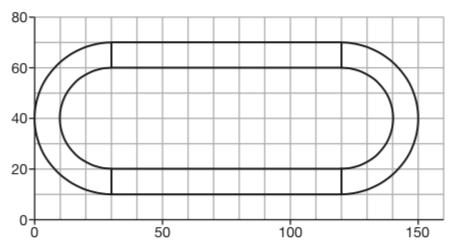
\includegraphics[width=0.6\textwidth]{path_Jan2019-31.png} \vspace{3cm}

\item A vendor is using an 8-ft by 8-ft tent for a craft fair. The legs of the tent are 9 ft tall and the top forms a square pyramid with a height of 3 ft.\\[1cm]
    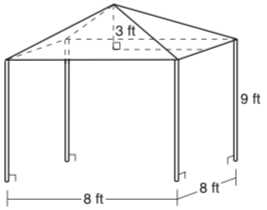
\includegraphics[width=0.4\textwidth]{tent_Jan2019-9.png}\\[0.5cm]
    What is the volume, in cubic feet, of space the tent occupies? \vspace{3cm}

\newpage
\item Sarah needs to replace two concrete sections in her sidewalk, as modeled below. Each section is 36 inches by 36 inches and 4 inches deep.\\[0.25cm]
    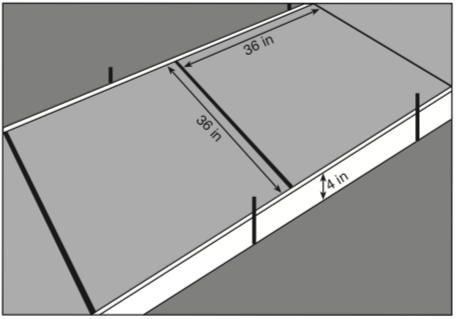
\includegraphics[width=0.5\textwidth]{walk_Aug2018-31.png}
      \begin{enumerate}
        \item Determine and state the volume of concrete needed, \emph{in cubic feet}. \vspace{1.5cm}
        \item Sarah can mix her own concrete for \$3.25 per cubic foot. How much money will it cost her to replace the two concrete sections?
    \end{enumerate} \vspace{2.5cm}

\item The greenhouse pictured below can be modeled as a rectangular prism with a half-cylinder on top. The rectangular prism is 20 feet wide, 12 feet high, and 45 feet long. The half-cylinder has a diameter of 20 feet.\\[0.5cm]
    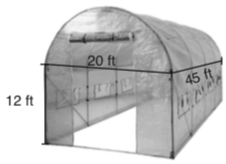
\includegraphics[width=0.3\textwidth]{greenhouse_Jun2018-7.png}\\
    To the \emph{nearest cubic foot}, what is the volume of the greenhouse?



\end{enumerate}
\end{document}